\cohead{\Large\textbf{Flächenberechnung}}
\fakesubsection{Berechnen von Flächen mit Hilfe von Integralen}
Eine häufig vorkommende Aufgabenstellung beginnt mit "Bestimme die Fläche, die\dots". Solche Aufgabenstellungen lassen sich mit Hilfe von Integralen lösen.
\begin{tcolorbox}[height=4cm]
	\textbf{Flächenberechnung}

	\textcolor{loestc}{Zur Flächenberechnung immer von Nullstelle (mit VZW) zu Nullstelle integrieren und die für die Flächen unterhalb der \(x\)-Achse den Wert von negativ auf positiv ändern.}
\end{tcolorbox}
Berechnen wir als Beispiel die von der Funktion \(f(x)=x^3-x^2-2x\) und der \(x\)-Achse eingeschlossenen Fläche:

\bigskip

\begin{minipage}{\textwidth}
	\adjustbox{valign=t}{\begin{minipage}{.6\textwidth}\raggedright
		\textcolor{loes}{Die Nullstellen können wir aus \(f(x)=0\) zu \(x_1=-1,\ x_2=0,\ x_3=2\) bestimmen.}
		\begin{align*}
			&\textcolor{loes}{\int\limits_{-1}^0 x^3-x^2-2x\td x=\frac{5}{12}}\\
			&\textcolor{loes}{\int\limits_{0}^2 x^3-x^2-2x\td x=-\frac{8}{3}}
		\end{align*}
		\textcolor{loes}{Der gesuchte Flächeninhalt hat also den Wert \(\frac{5}{12}+\frac{8}{3}=\frac{37}{12}\)}
	\end{minipage}}%
	\adjustbox{valign=t, padding = 3ex 0ex 0ex 0ex}{\begin{minipage}{.4\textwidth-3ex}
		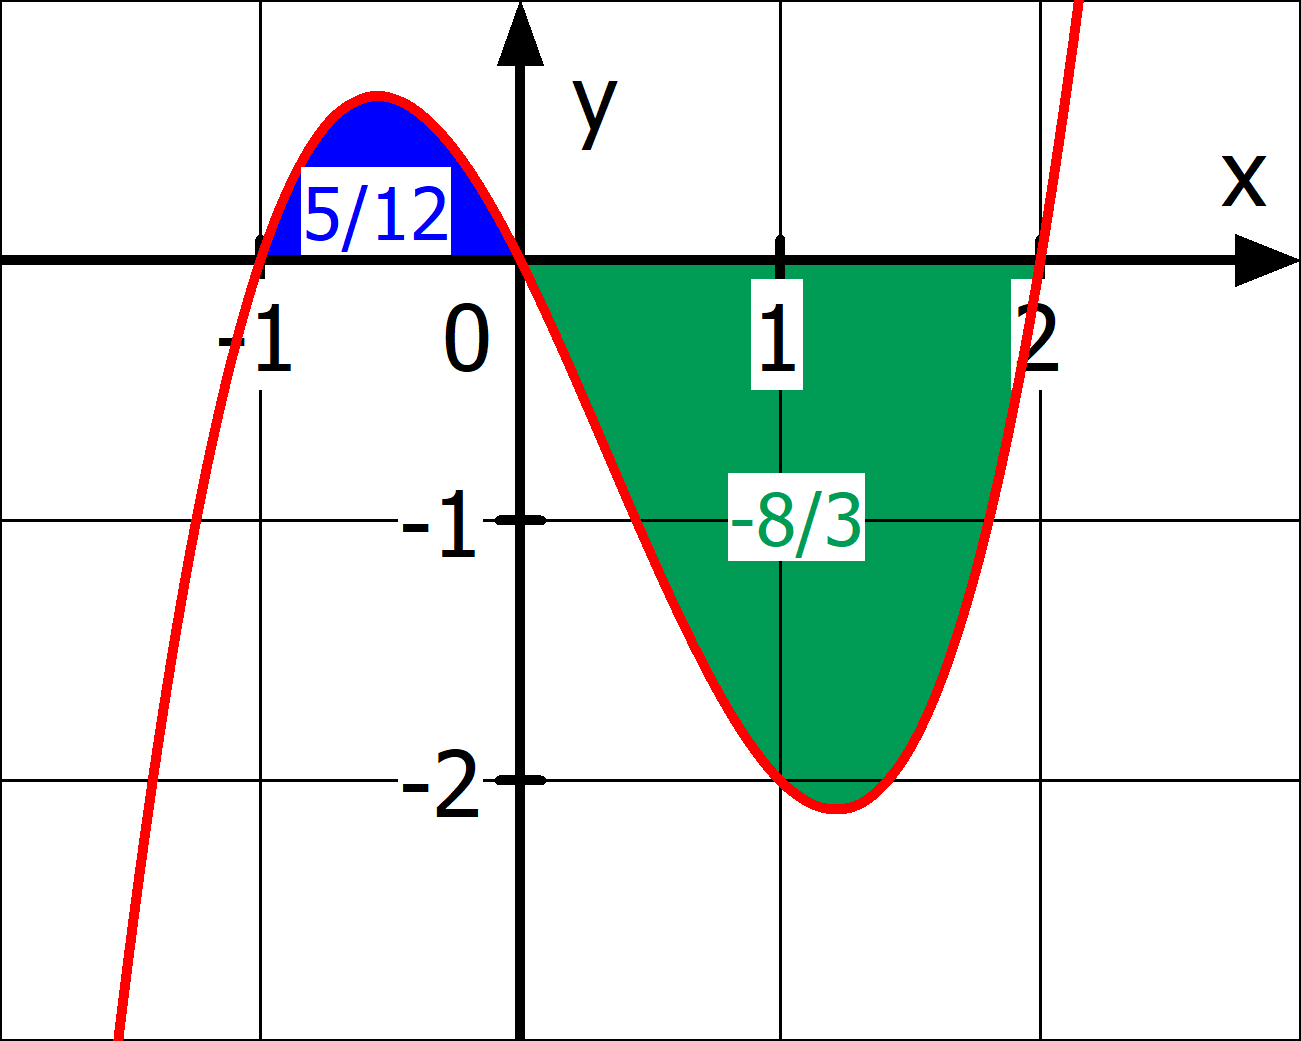
\includegraphics[width=\linewidth]{\integration/pics/bsp_flaeche.png}
	\end{minipage}}%
\end{minipage}

\bigskip

Bestimme die von der Funktion  \(f(x)=\frac{1}{2}e^{\ln(2)x}-4\), der \(x\)-Achse und der \(y\)-Achse eingeschlossene Fläche:

\bigskip

\begin{minipage}{\textwidth}
	\adjustbox{valign=t, padding = 0ex 0ex 3ex 0ex}{\begin{minipage}{.4\textwidth-3ex}
		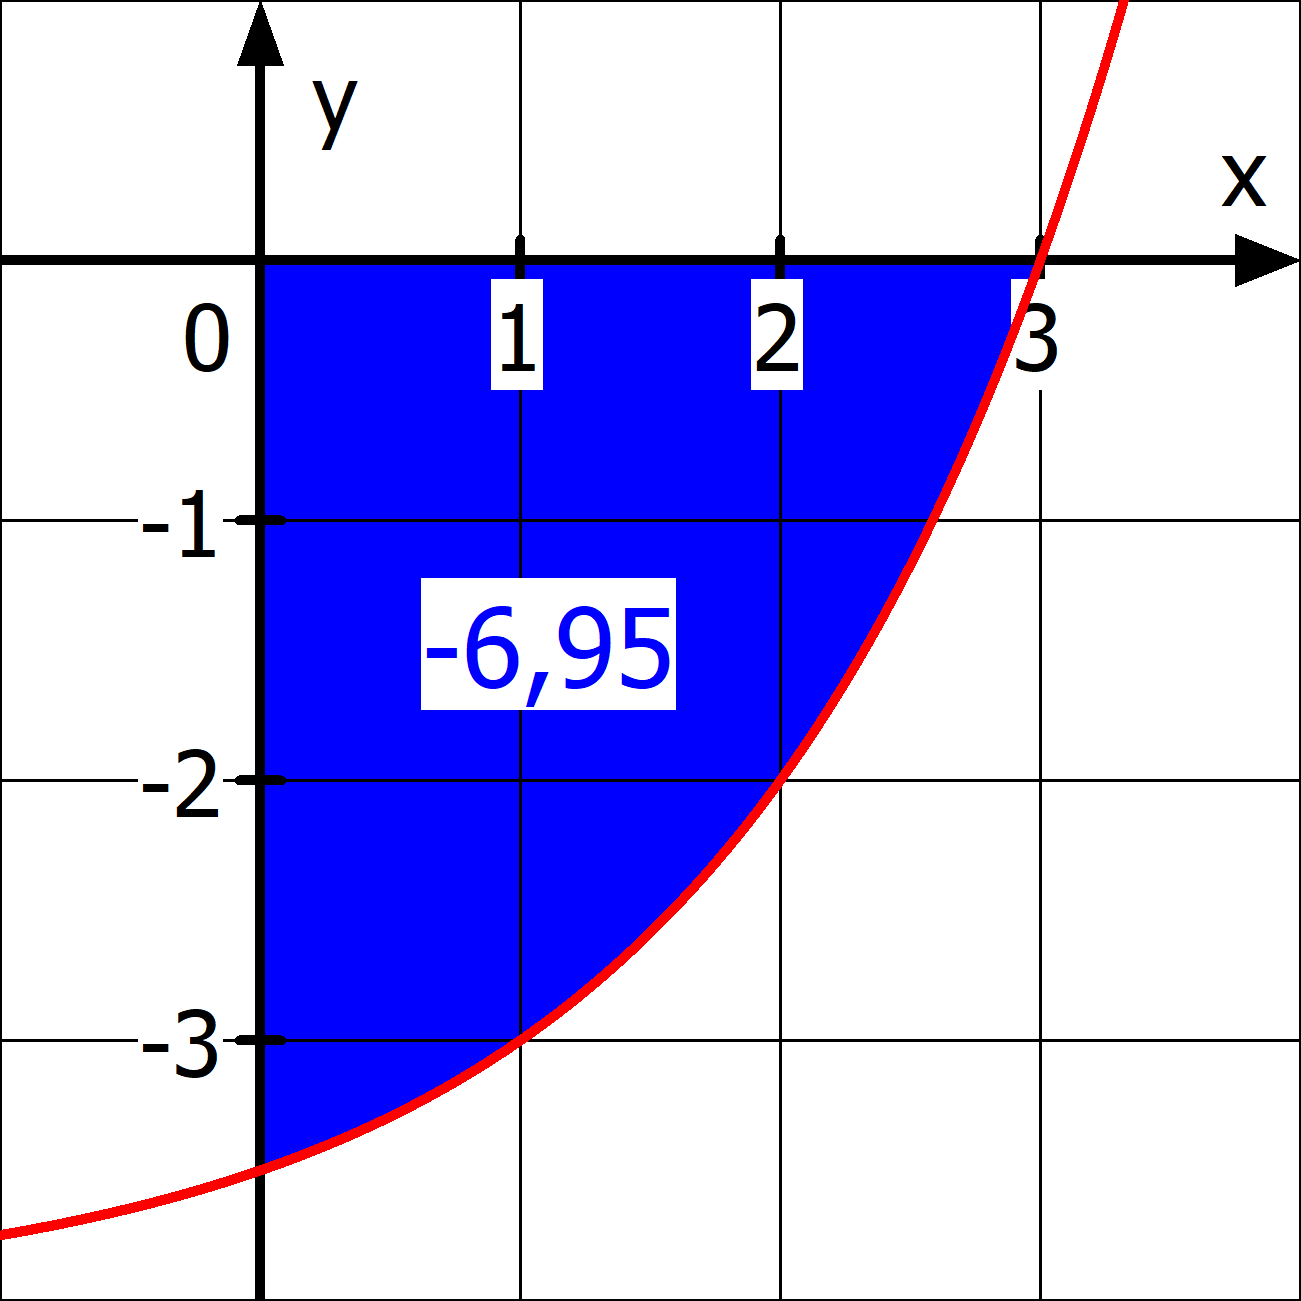
\includegraphics[width=\linewidth]{\integration/pics/bsp_flaeche2.png}
	\end{minipage}}%
	\adjustbox{valign=t}{\begin{minipage}{.6\textwidth}\raggedright
		\textcolor{loes}{Die Nullstelle können wir aus \(f(x)=0\) zu \(x_1=3\) bestimmen.}
		\begin{align*}
			&\textcolor{loes}{\int\limits_{0}^3 \tfrac{1}{2}e^{\ln(2)x}-4\td x=\frac{7}{2\ln(2)}-12\approx -6,95}
		\end{align*}
		\textcolor{loes}{Der gesuchte Flächeninhalt hat also den Wert \(-\int\limits_{0}^3 \tfrac{1}{2}e^{\ln(2)x}-4\td x\approx 6,95\)}
	\end{minipage}}%
\end{minipage}
\newpage
\begin{minipage}{\textwidth}\vspace{-\baselineskip}
	\adjustbox{valign=t, padding = 0ex 0ex 2ex 0ex}{\begin{minipage}{.5\textwidth-2ex}
        \begin{Exercise}[title={\raggedright\normalfont Berechne jeweils die von der Funktion und der \(x\)-Achse eingeschlossene Fläche.}, label=flaecheRechnA1]
			\begin{enumerate}[label=\alph*)]
				\item \(f(x)=x^3+2x^2-8x\)
				\item \(f(x)=-\frac{1}{3}x^3+x^2+6x\)
				\item \(f(x)=x^4+x^2-2\)
				\item \(f(x)=-2x^3-4x^2+6x\)
				\item \(f(x)=-4x^3-12x^2+40x\)
				\item \(f(x)=2x^3-11x^2+12x\)
				\item \(f(x)=-x^6+7x^3+8\)
				\item \(f(x)=-2x^4-3,5x^2+18\)
				\item \(f(x)=1,5x^4-7,5x^2+6\)
				\item \(f(x)=\frac{5}{3}x^7-\frac{37}{3}x^4-\frac{40}{3}x\)
			\end{enumerate}
		\end{Exercise}
	\end{minipage}}%
	\adjustbox{valign=t, padding = 2ex 0ex 0ex 0ex}{\begin{minipage}{.5\textwidth-2ex}
		\begin{Exercise}[title={\raggedright\normalfont Berechne jeweils die von der Funktion und den Koordinatenachsen eingeschlossene Fläche.}, label=flaecheRechnA2]
			\begin{enumerate}[label=\alph*)]
				\item \(f(x)=8e^{2x}-4\)
				\item \(f(x)=-3e^{0,5x}+5\)
				\item \(f(x)=-5e^{\tfrac{1}{4}x}+1\)
				\item \(f(x)=-3e^{\tfrac{3}{5}x}+8\)
				\item \(f(x)=\tfrac{7}{4}e^{\tfrac{2}{7}x}-6\)
				\item \(f(x)=-4e^{-2x}+0,1\)
				\item \(f(x)=-3e^{-x}+5\)
				\item \(f(x)=-e^{\tfrac{1}{3}x}+0,5\)
				\item \(f(x)= 3e^{0,2x}-9\)
				\item \(f(x)=-2e^{0,1x}+1\)
			\end{enumerate}
		\end{Exercise}
	\end{minipage}}%
\end{minipage}
%%%%%%%%%%%%%%%%%%%%%%%%%%%%%%%%%%%%%%%%%
\begin{Answer}[ref=flaecheRechnA1]
	\begin{enumerate}[label=\alph*)]
		\item \(\displaystyle\int\limits_{-4}^{0} x^3+2x^2-8x\td x-\int\limits_{0}^{2} x^3+2x^2-8x\td=\frac{128}{3}+\frac{20}{3}=\frac{148}{3}\)
		\item \(\displaystyle-\int\limits_{-3}^{0} -\frac{1}{3}x^3+x^2+6x\td x+\int\limits_{0}^{6} -\frac{1}{3}x^3+x^2+6x\td x=\frac{45}{4}+72=\frac{333}{4}\)
		\item \(\displaystyle-\int\limits_{-1}^{1} x^4+x^2-2\td x=\frac{44}{15}\)
		\item \(\displaystyle-\int\limits_{-3}^{0} -2x^3-4x^2+6x\td x+\int\limits_{0}^{1} -2x^3-4x^2+6x\td x=\frac{45}{2}+\frac{7}{6}=\frac{71}{3}\)
		\item \(\displaystyle -\int\limits_{-5}^{0}-4x^3-12x^2+40x \td x +\int\limits_{0}^{2}-4x^3-12x^2+40x \td x=375+32=407\)
		\item \(\displaystyle \int\limits_{0}^{\tfrac{3}{2}} 2x^3-11x^2+12x \td x - \int\limits_{\tfrac{3}{2}}^{4} 2x^3-11x^2+12x \td x=\frac{117}{32}+\frac{1375}{96}=\frac{863}{48}\)
		\item \(\displaystyle -\int\limits_{-1}^{2} -x^6+7x^3+8 \td x=\frac{891}{28}\)
		\item \(\displaystyle -\int\limits_{-1,5}^{1,5} -2x^4-3,5x^2+18 \td x=40,05\)
		\item \(\displaystyle-\int\limits_{-2}^{-1} 1,5x^4-7,5x^2+6\td x+\int\limits_{-1}^{1} 1,5x^4-7,5x^2+6\td x-\int\limits_{1}^{2} 1,5x^4-7,5x^2+6\td x=2,2+7,6+2,2=12\)
		\item \(\displaystyle \int\limits_{-1}^{0} \frac{5}{3}x^7-\frac{37}{3}x^4-\frac{40}{3}x \td x-\int\limits_{0}^{2} \frac{5}{3}x^7-\frac{37}{3}x^4-\frac{40}{3}x \td x=\frac{33}{8}+48=\frac{417}{8}\)
	\end{enumerate}
\end{Answer}
\begin{Answer}[ref=flaecheRechnA2]
	\begin{enumerate}[label=\alph*)]
		\item \(\displaystyle-\int\limits_{\frac{\ln(2)}{2}}^{0} 8e^{2x}-4 \td x=2-2\ln(2)\approx 0,61\)
		\item \(\displaystyle\int\limits_{-2\ln\left(\tfrac{5}{3}\right)}^{0} -3e^{0,5x}+5 \td x=4-10\ln\left(\tfrac{5}{3}\right)\approx1,11\)
		\item \(\displaystyle-\int\limits_{4\ln\left(\tfrac{1}{5}\right)}^{0} -5e^{\tfrac{1}{4}x}+1 \td x=16+4\ln\left(\tfrac{1}{5}\right)\approx 9,56\)
		\item \(\displaystyle\int\limits_{0}^{\tfrac{5}{3}\ln\left(\tfrac{8}{3}\right)} -3e^{\tfrac{3}{5}x}+8 \td x=-\tfrac{28}{3}+\tfrac{40}{3}\ln\left(\tfrac{8}{3}\right)\approx 3,74\)
		\item \(\displaystyle-\int\limits_{0}^{\tfrac{7}{2}\ln\left(\tfrac{24}{7}\right)} \tfrac{7}{4}e^{\tfrac{2}{7}x}-6 \td x=-\tfrac{119}{8}+21\ln\left(\tfrac{24}{7}\right)\approx 11,00\)
		\item \(\displaystyle-\int\limits_{0}^{-0,5\ln(0,025x)} -4e^{-2x}+0,1 \td x= 1,95+0,05\ln(0,025)\approx 1,77\)
		\item \(\displaystyle\int\limits_{-\ln\left(\tfrac{5}{3}\right)}^{0} -3e^{-x}+5 \td x=-2+5\ln\left(\tfrac{5}{3}\right)\approx 0,55\)
		\item \(\displaystyle\int\limits_{3\ln(0,5)}^{0} -e^{\tfrac{1}{3}x}+0,5 \td x=1,5+1,5\ln(0,5)\approx 0,46\)
		\item \(\displaystyle-\int\limits_{0}^{5\ln(3)} 3e^{0,2x}-9 \td x=-30+45\ln(3)\approx 19,44\)
		\item \(\displaystyle-\int\limits_{10\ln(0,5)}^{0} -2e^{0,1x}+1 \td x=10+10\ln(0,5)\approx 3,07\)
	\end{enumerate}
\end{Answer}